\documentclass[11pt,a4paper]{report}
\usepackage[textwidth=37em,vmargin=30mm]{geometry}
\usepackage{calc,xunicode,amsmath,amssymb,paralist,enumitem,tabu,booktabs,datetime2,xeCJK,xeCJKfntef,listings}
\usepackage{tocloft,fancyhdr,tcolorbox,xcolor,graphicx,eso-pic,xltxtra,xelatexemoji}

\newcommand{\envyear}[0]{2025}
\newcommand{\envdatestr}[0]{2025-07-13}
\newcommand{\envfinaldir}[0]{webdb/2025/20250713/final}

\usepackage[hidelinks]{hyperref}
\hypersetup{
    colorlinks=false,
    pdfpagemode=FullScreen,
    pdftitle={Web Digest - \envdatestr}
}

\setlength{\cftbeforechapskip}{10pt}
\renewcommand{\cftchapfont}{\rmfamily\bfseries\large\raggedright}
\setlength{\cftbeforesecskip}{2pt}
\renewcommand{\cftsecfont}{\sffamily\small\raggedright}

\setdefaultleftmargin{2em}{2em}{1em}{1em}{1em}{1em}

\usepackage{xeCJK,xeCJKfntef}
\xeCJKsetup{PunctStyle=plain,RubberPunctSkip=false,CJKglue=\strut\hskip 0pt plus 0.1em minus 0.05em,CJKecglue=\strut\hskip 0.22em plus 0.2em}
\XeTeXlinebreaklocale "zh"
\XeTeXlinebreakskip = 0pt


\setmainfont{Brygada 1918}
\setromanfont{Brygada 1918}
\setsansfont{IBM Plex Sans}
\setmonofont{JetBrains Mono NL}
\setCJKmainfont{Noto Serif CJK SC}
\setCJKromanfont{Noto Serif CJK SC}
\setCJKsansfont{Noto Sans CJK SC}
\setCJKmonofont{Noto Sans CJK SC}

\setlength{\parindent}{0pt}
\setlength{\parskip}{8pt}
\linespread{1.15}

\lstset{
	basicstyle=\ttfamily\footnotesize,
	numbersep=5pt,
	backgroundcolor=\color{black!5},
	showspaces=false,
	showstringspaces=false,
	showtabs=false,
	tabsize=2,
	captionpos=b,
	breaklines=true,
	breakatwhitespace=true,
	breakautoindent=true,
	linewidth=\textwidth
}






\newcommand{\coverpic}[2]{
    % argv: itemurl, authorname
    Cover photo by #2~~(\href{#1}{#1})
}
\newcommand{\makeheader}[0]{
    \begin{titlepage}
        % \newgeometry{hmargin=15mm,tmargin=21mm,bmargin=12mm}
        \begin{center}
            
            \rmfamily\scshape
            \fontspec{BaskervilleF}
            \fontspec{Old Standard}
            \fontsize{59pt}{70pt}\selectfont
            WEB\hfill DIGEST
            
            \vfill
            % \vskip 30pt
            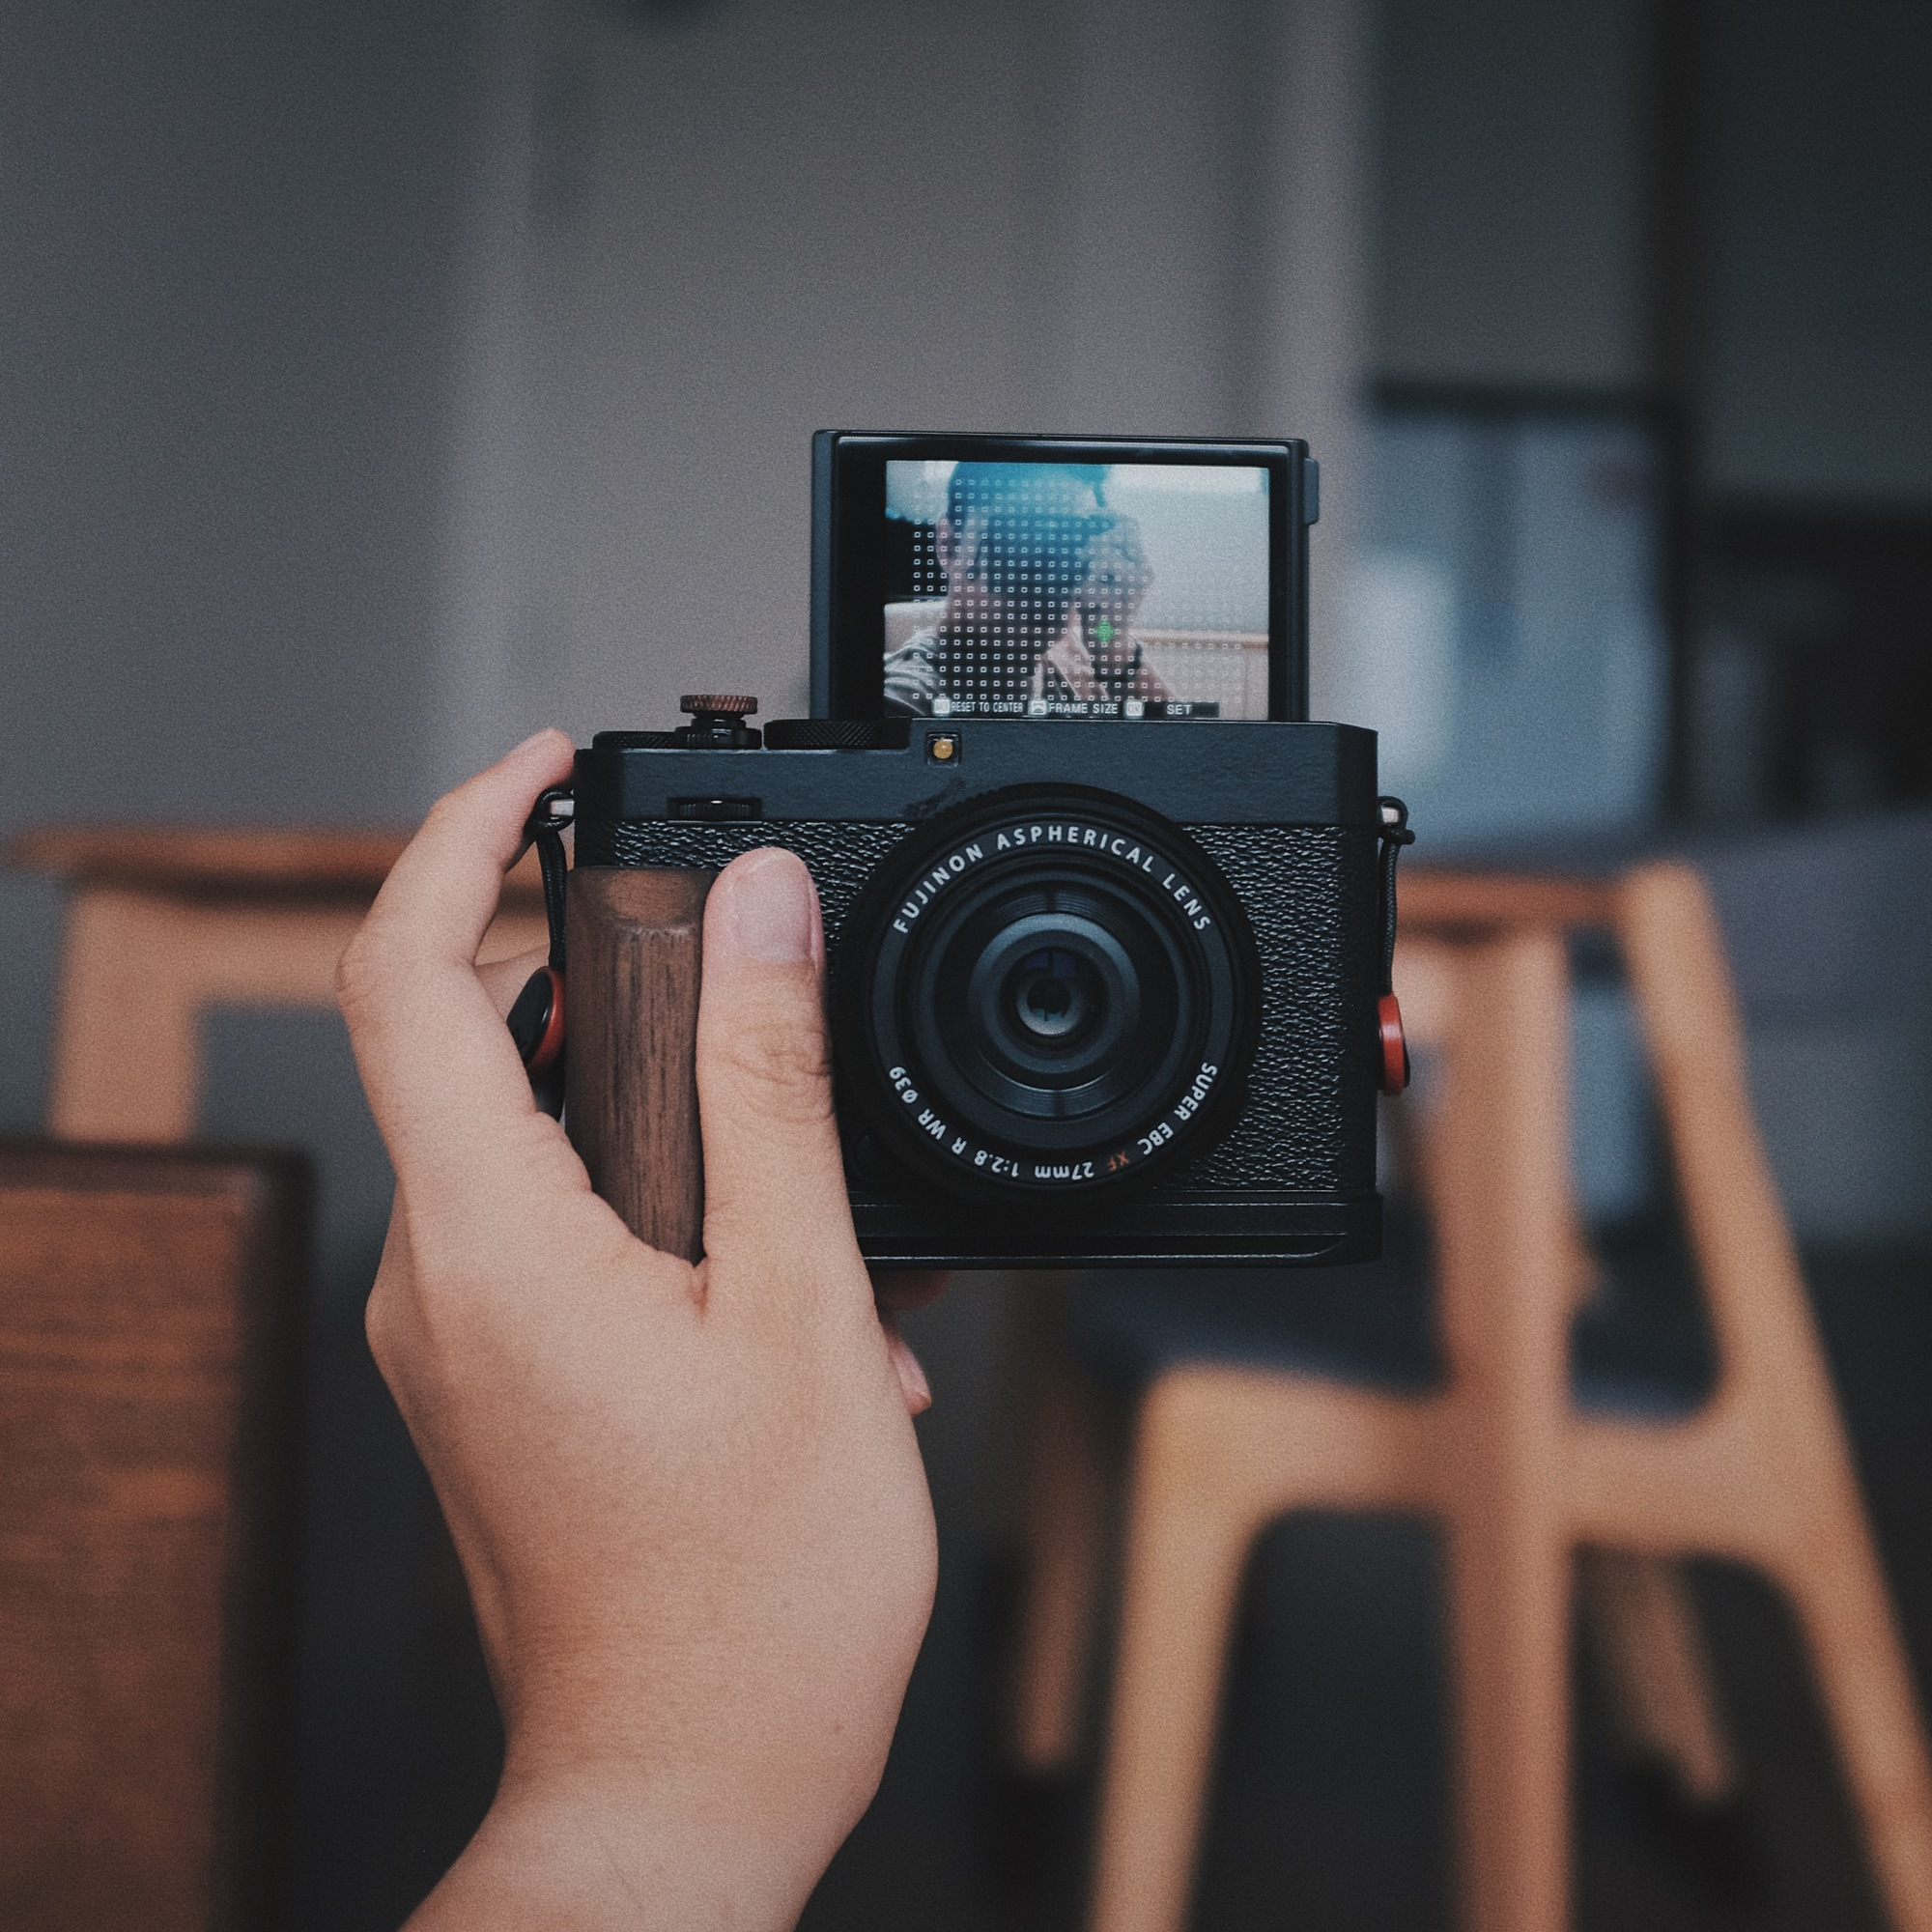
\includegraphics[width=\linewidth]{\envfinaldir/coverpic-prod.jpg}\par
            % \vskip 30pt
            \vfill

            \normalsize\rmfamily\scshape
            \copyright{} The Web Digest Project \hfill\large \envdatestr
        \end{center}
    \end{titlepage}
    % \restoregeometry
}
\newcommand{\simplehref}[1]{%
    \textcolor{blue!80!green}{\href{#1}{#1}}%
}
\renewcommand{\contentsname}{\center\Huge\sffamily\bfseries Contents\par\vskip 20pt}
\newcounter{ipartcounter}
\setcounter{ipartcounter}{0}
\newcommand{\ipart}[1]{
    % \vskip 20pt
    \clearpage
    \stepcounter{ipartcounter}
    \phantomsection
    \addcontentsline{toc}{chapter}{#1}
    % \begin{center}
    %     \Huge
    %     \sffamily\bfseries
    %     #1
    % \end{center}
    % \vskip 20pt plus 7pt
}
\newcounter{ichaptercounter}
\setcounter{ichaptercounter}{0}
\newcommand{\ichapter}[1]{
    % \vskip 20pt
    \clearpage
    \stepcounter{ichaptercounter}
    \phantomsection
    \addcontentsline{toc}{section}{\numberline{\arabic{ichaptercounter}}#1}
    \begin{center}
        \Huge
        \sffamily\bfseries
        #1
    \end{center}
    \vskip 20pt plus 7pt
}
\newcommand{\entrytitlefont}[1]{\subsection*{\raggedright\Large\sffamily\bfseries#1}}
\newcommand{\entryitemGeneric}[2]{
    % argv: title, url
    \parbox{\linewidth}{
        \entrytitlefont{#1}\par\vskip 5pt
        \footnotesize\ttfamily\mdseries
        \simplehref{#2}
    }\vskip 11pt plus 11pt minus 1pt
}
\newcommand{\entryitemGithub}[3]{
    % argv: title, url, desc
    \parbox{\linewidth}{
        \entrytitlefont{#1}\par\vskip 5pt
        \footnotesize\ttfamily\mdseries
        \simplehref{#2}\par\vskip 5pt
        \small\rmfamily\mdseries#3
    }\vskip 11pt plus 11pt minus 1pt
}
\newcommand{\entryitemAp}[3]{
    % argv: title, url, desc
    \parbox{\linewidth}{
        \entrytitlefont{#1}\par\vskip 5pt
        \footnotesize\ttfamily\mdseries
        \simplehref{#2}\par\vskip 5pt
        \small\rmfamily\mdseries#3
    }\vskip 11pt plus 11pt minus 1pt
}
\newcommand{\entryitemHackernews}[3]{
    % argv: title, hnurl, rawurl
    % \parbox{\linewidth}{
    %     \entrytitlefont{#1}\par\vskip 5pt
    %     \footnotesize\ttfamily\mdseries
    %     \simplehref{#3}\par
    %     \textcolor{black!50}{\href{#2}{#2}}
    % }\vskip 11pt plus 11pt minus 1pt
    \begin{minipage}{\linewidth}
            \entrytitlefont{#1}\par\vskip 5pt
            \footnotesize\ttfamily\mdseries
            \simplehref{#3}\par
            \textcolor{black!50}{\href{#2}{#2}}
    \end{minipage}\par\vskip 11pt plus 11pt minus 1pt
}







\begin{document}

\makeheader

\tableofcontents\clearpage




\ipart{Developers}
\ichapter{Hacker News}
\entryitemTwoLinks{Bypassing Google's big anti-adblock update}{https://news.ycombinator.com/item?id=44544266}{https://0x44.xyz/blog/web-request-blocking/}

\entryitemTwoLinks{Supreme Court's ruling practically wipes out free speech for sex writing online}{https://news.ycombinator.com/item?id=44543865}{https://ellsberg.substack.com/p/free-speech}

\entryitemTwoLinks{Kimi k2 largest open source SOTA model?}{https://news.ycombinator.com/item?id=44543508}{https://github.com/MoonshotAI/Kimi-K2}

\entryitemTwoLinks{Arizona resident dies from the plague less than 24 hours after showing symptoms}{https://news.ycombinator.com/item?id=44543368}{https://www.independent.co.uk/news/health/arizona-plague-death-cases-b2787325.html}

\entryitemTwoLinks{Proposed NOAA Budget Kills Program Designed to Prevent Satellite Collisions}{https://news.ycombinator.com/item?id=44543150}{https://skyandtelescope.org/astronomy-news/proposed-noaa-budget-kills-program-to-prevent-satellite-collisions/}

\entryitemTwoLinks{Vibe-Coding a PCB – surprisingly good}{https://news.ycombinator.com/item?id=44542880}{https://atomic14.substack.com/p/vibe-coding-a-pcb-surprisingly-good}

\entryitemTwoLinks{The fish kick may be the fastest subsurface swim stroke yet (2015)}{https://news.ycombinator.com/item?id=44541576}{https://nautil.us/is-this-new-swim-stroke-the-fastest-yet-235511/}

\entryitemTwoLinks{Working through 'Writing A C Compiler'}{https://news.ycombinator.com/item?id=44541565}{https://jollygoodsw.wordpress.com/2025/03/13/working-through-writing-a-c-compiler/}

\entryitemTwoLinks{ICANN fumes as AFRINIC offers no explanation for annulled election}{https://news.ycombinator.com/item?id=44540858}{https://www.theregister.com/2025/07/11/afrinic\_election\_annulled\_why/}

\entryitemTwoLinks{Commodore 64 Ultimate}{https://news.ycombinator.com/item?id=44540589}{https://www.commodore.net}

\entryitemTwoLinks{MacPaint Art from the Mid-80s Still Looks Great Today}{https://news.ycombinator.com/item?id=44540402}{https://blog.decryption.net.au/posts/macpaint.html}

\entryitemTwoLinks{New Date("wtf") – How well do you know JavaScript's Date class?}{https://news.ycombinator.com/item?id=44540241}{https://jsdate.wtf}

\entryitemTwoLinks{Bad Actors Are Grooming LLMs to Produce Falsehoods}{https://news.ycombinator.com/item?id=44540052}{https://americansunlight.substack.com/cp/168074209}

\entryitemTwoLinks{Malware found in official gravityforms plugin indicating supply chain breach}{https://news.ycombinator.com/item?id=44539879}{https://patchstack.com/articles/critical-malware-found-in-gravityforms-official-plugin-site/}

\entryitemTwoLinks{Incus – Next-generation system container, application container, and VM manager}{https://news.ycombinator.com/item?id=44539338}{https://linuxcontainers.org/incus/}

\entryitemTwoLinks{FEMA Didn't Answer Thousands of Calls From Flood Survivors}{https://news.ycombinator.com/item?id=44538923}{https://www.nytimes.com/2025/07/11/climate/fema-missed-calls-texas-floods.html}

\entryitemTwoLinks{Replication of Quantum Factorisation Records with an 8-bit Home Computer [pdf]}{https://news.ycombinator.com/item?id=44538693}{https://eprint.iacr.org/2025/1237.pdf}

\entryitemTwoLinks{Tell HN: uBlock Origin on Chrome is finally gone}{https://news.ycombinator.com/item?id=44538517}{https://news.ycombinator.com/item?id=44538517}

\entryitemTwoLinks{OpenAI delays launch of open-weight model}{https://news.ycombinator.com/item?id=44538413}{https://twitter.com/sama/status/1943837550369812814}

\entryitemTwoLinks{Faking a JPEG}{https://news.ycombinator.com/item?id=44537631}{https://www.ty-penguin.org.uk/~auj/blog/2025/03/25/fake-jpeg/}


\ipart{Developers~~~~(zh-Hans)}
\ichapter{Solidot}
\entryitemGeneric{\hskip 0pt{}海洋中的纳米塑料多达数千万吨}{https://www.solidot.org/story?sid=81770}

\entryitemGeneric{\hskip 0pt{}GlobalFoundries 收购 MIPS}{https://www.solidot.org/story?sid=81769}

\entryitemGeneric{\hskip 0pt{}《星露谷物语》成为 Steam 平台最受好评的游戏}{https://www.solidot.org/story?sid=81768}

\entryitemGeneric{\hskip 0pt{}只有 1\% 的龟罹患癌症}{https://www.solidot.org/story?sid=81767}

\entryitemGeneric{\hskip 0pt{}Amarok 3.3 释出}{https://www.solidot.org/story?sid=81766}

\entryitemGeneric{\hskip 0pt{}基因组研究确认人类圈养动物后动物病毒开始传播给人类}{https://www.solidot.org/story?sid=81765}

\entryitemGeneric{\hskip 0pt{}西欧经历有记录以来最热的六月}{https://www.solidot.org/story?sid=81764}

\entryitemGeneric{\hskip 0pt{}两性权力关系泾渭并不分明}{https://www.solidot.org/story?sid=81763}

\entryitemGeneric{\hskip 0pt{}OpenAI 将发布 AI Web 浏览器挑战 Chrome  }{https://www.solidot.org/story?sid=81762}

\entryitemGeneric{\hskip 0pt{}麦当劳的 AI 招聘平台管理员密码是 123456}{https://www.solidot.org/story?sid=81761}

\entryitemGeneric{\hskip 0pt{}英伟达市值突破 4 万亿美元}{https://www.solidot.org/story?sid=81760}

\entryitemGeneric{\hskip 0pt{}美国科技巨头对财政部的制裁名单响应并不迅速}{https://www.solidot.org/story?sid=81759}\ichapter{V2EX}
\entryitemGeneric{\hskip 0pt{}[问与答] 野卡跑了还有什么虚拟卡替代品呢?有靠谱点的没?}{https://www.v2ex.com/t/1144846}

\entryitemGeneric{\hskip 0pt{}[职场话题] 4 年前我转行做销售了,去年拿了销冠}{https://www.v2ex.com/t/1144843}

\entryitemGeneric{\hskip 0pt{}[Claude] 国内 Vibe Coding:基于 Kimi K2 的 Claude Code Docker 版}{https://www.v2ex.com/t/1144842}

\entryitemGeneric{\hskip 0pt{}[微信] 用了十多年的 wechat 说登陆不上就登不上了。}{https://www.v2ex.com/t/1144841}

\entryitemGeneric{\hskip 0pt{}[iDev] XCode 的 7 日签名有办法不借助第三方工具,写个脚本在有效期<1 天时自动重签吗?默认好像要过期了才能重签。自己开的 App,不打算上架,不想注册开发者账号}{https://www.v2ex.com/t/1144840}

\entryitemGeneric{\hskip 0pt{}[分享发现] 新加坡地铁图 - 全面指南与网络布局}{https://www.v2ex.com/t/1144835}

\entryitemGeneric{\hskip 0pt{}[Claude] 在 Windows 上使用 Claude Code 不再需要 WSL 环境了}{https://www.v2ex.com/t/1144834}

\entryitemGeneric{\hskip 0pt{}[路由器] 求助! passwall+adguard 电脑版 有的网站打不开}{https://www.v2ex.com/t/1144832}

\entryitemGeneric{\hskip 0pt{}[程序员] [经验分享] Kimi K2 发布,我用 Kimi K2 替换了 Claude Code 默认模型}{https://www.v2ex.com/t/1144831}

\entryitemGeneric{\hskip 0pt{}[酷工作] Alphaist 新兴美元基金| AI 投资全职/实习生、品牌内容全职/实习生招募}{https://www.v2ex.com/t/1144829}

\entryitemGeneric{\hskip 0pt{}[分享创造] Claude code 30 分钟做了一个 Kimi k2 免费套壳站}{https://www.v2ex.com/t/1144828}

\entryitemGeneric{\hskip 0pt{}[Cursor] Cursor 老用户可切回旧套餐了}{https://www.v2ex.com/t/1144827}

\entryitemGeneric{\hskip 0pt{}[NAS] 推荐一个好用的 NAS 系统:飞牛,欢迎交流}{https://www.v2ex.com/t/1144825}

\entryitemGeneric{\hskip 0pt{}[浏览器] Jiffy Reader 发生了什么?}{https://www.v2ex.com/t/1144823}

\entryitemGeneric{\hskip 0pt{}[Apple] 准备买个 TCL 75-Inch Class QM7K Series QD-Mini LED 4K UHD Google Smart TV(海外版),求问建议配 Apple TV 吗?}{https://www.v2ex.com/t/1144822}

\entryitemGeneric{\hskip 0pt{}[程序员] 中国就是因为想掌握``驭人之术''的这种人太多了,才会是现在这种屌样子}{https://www.v2ex.com/t/1144819}

\entryitemGeneric{\hskip 0pt{}[问与答] 如何才能判断自己是否擅长一件事}{https://www.v2ex.com/t/1144818}

\entryitemGeneric{\hskip 0pt{}[上海] In a world that won't stop spinning, find your center.}{https://www.v2ex.com/t/1144817}

\entryitemGeneric{\hskip 0pt{}[酷工作] 招聘(远程办公): DevOps 工程师 Flutter(app) Golang  测试工程师 前端工程师(Nodejs / React) 大数据开发工程师 Product Manager}{https://www.v2ex.com/t/1144816}

\entryitemGeneric{\hskip 0pt{}[问与答] tplink 路由器真的搞不了智能家居}{https://www.v2ex.com/t/1144814}

\entryitemGeneric{\hskip 0pt{}[问与答] Gemini api 使用接口限速怎么回事?我是付款账户啊 ? gemini-2.5-flash}{https://www.v2ex.com/t/1144813}

\entryitemGeneric{\hskip 0pt{}[Surge] Surge 5 版本疑惑}{https://www.v2ex.com/t/1144811}

\entryitemGeneric{\hskip 0pt{}[MacBook Air] 第一次用 m 芯片的 macbook 有需要注意的地方吗?}{https://www.v2ex.com/t/1144810}

\entryitemGeneric{\hskip 0pt{}[问与答] Edge 弹广告,有人遇到吗?}{https://www.v2ex.com/t/1144808}

\entryitemGeneric{\hskip 0pt{}[生活] 大家今天过的怎样}{https://www.v2ex.com/t/1144807}

\entryitemGeneric{\hskip 0pt{}[分享发现] 分享下窦唯的纯音乐,合集下面有十个专辑}{https://www.v2ex.com/t/1144805}

\entryitemGeneric{\hskip 0pt{}[问与答] [不懂就问] 有没有无限制的开源大模型?}{https://www.v2ex.com/t/1144803}

\entryitemGeneric{\hskip 0pt{}[问与答] 导航用的高精地图哪里能找到}{https://www.v2ex.com/t/1144802}

\entryitemGeneric{\hskip 0pt{}[问与答] 国家不是说学位证不再要求英语水平了吗,为什么现在专升本想拿学位证还要求考学位英语?}{https://www.v2ex.com/t/1144801}

\entryitemGeneric{\hskip 0pt{}[奇思妙想] 租房客一般不在小区业主群里,很多停水停电信息收不到,有无简易办法,比如注册个小程序,物业发消息时也通知小程序,小程序通过服务号广播给订阅的人}{https://www.v2ex.com/t/1144800}

\entryitemGeneric{\hskip 0pt{}[宽带症候群] AC+AP 的这个问题怎么从来没人提过?}{https://www.v2ex.com/t/1144799}

\entryitemGeneric{\hskip 0pt{}[酷工作] [郑州地区寻找兼职] CRUD 兼职,技术栈 springboot / vue3 / miniapp}{https://www.v2ex.com/t/1144796}

\entryitemGeneric{\hskip 0pt{}[求职] 38 岁的 Java 老人求职还有救吗?}{https://www.v2ex.com/t/1144795}

\entryitemGeneric{\hskip 0pt{}[VXNA] 申请收录 blog:一叶斋}{https://www.v2ex.com/t/1144794}

\entryitemGeneric{\hskip 0pt{}[问与答] 各位大佬们,还有什么 chatgpt api 付款的路子推荐嘛}{https://www.v2ex.com/t/1144793}

\entryitemGeneric{\hskip 0pt{}[随想] 无论你去了哪里,都要全心全意的去。}{https://www.v2ex.com/t/1144791}

\entryitemGeneric{\hskip 0pt{}[分享创造] 用 ai 做的第一个 ai web 应用 [人脸贴 emoji] 欢迎使用和拍砖}{https://www.v2ex.com/t/1144789}

\entryitemGeneric{\hskip 0pt{}[分享发现] 给大家推荐一个打发时间的在线拼图网站}{https://www.v2ex.com/t/1144788}

\entryitemGeneric{\hskip 0pt{}[旅行] 简单分享一下十二天的法意瑞旅行,行程表和开销 [多图]}{https://www.v2ex.com/t/1144787}

\entryitemGeneric{\hskip 0pt{}[北京] 又练了 5 小时的高速和山路,开的丝滑了也想买车了}{https://www.v2ex.com/t/1144786}

\entryitemGeneric{\hskip 0pt{}[问与答] 有没有资讯聚合终端或者网站推荐?}{https://www.v2ex.com/t/1144785}

\entryitemGeneric{\hskip 0pt{}[职场话题] 7 月是招聘淡季吗?}{https://www.v2ex.com/t/1144784}

\entryitemGeneric{\hskip 0pt{}[路由器] 华硕路由器的固件支持动态路由协议吗?}{https://www.v2ex.com/t/1144782}

\entryitemGeneric{\hskip 0pt{}[分享创造] 揽佬最近很火, vibe coding 了一个找歌词的网站}{https://www.v2ex.com/t/1144781}

\entryitemGeneric{\hskip 0pt{}[硬件] 新手装机求指导}{https://www.v2ex.com/t/1144780}

\entryitemGeneric{\hskip 0pt{}[问与答] windows 有什么好用的启动器吗?}{https://www.v2ex.com/t/1144779}

\entryitemGeneric{\hskip 0pt{}[全球工单系统] 爱普生打印机就是个垃圾,赞同的来安慰一个}{https://www.v2ex.com/t/1144778}

\entryitemGeneric{\hskip 0pt{}[程序员] 意见征集,做个给 claude, gemini 提供上下文的 browser \& node line tracer 有人愿意购买吗}{https://www.v2ex.com/t/1144775}

\entryitemGeneric{\hskip 0pt{}[投资] 创建了个大 a 投资交流群}{https://www.v2ex.com/t/1144774}

\entryitemGeneric{\hskip 0pt{}[分享发现] 野卡的国内关联企业 海南莱成玖}{https://www.v2ex.com/t/1144772}


\ipart{Generic News}







\clearpage
\leavevmode\vfill
\footnotesize

Copyright \copyright{} 2023-2025 Neruthes and other contributors.

This document is published with CC BY-NC-ND 4.0 license.

The entries listed in this newsletter may be copyrighted by their respective creators.

This newsletter is generated by the Web Digest project.

The newsletters are also delivered via Telegram channel \CJKunderline{\href{https://t.me/webdigestchannel}{https://t.me/webdigestchannel}}.\\
RSS feed is available at \CJKunderline{\href{https://webdigest.pages.dev/rss.xml}{https://webdigest.pages.dev/rss.xml}}.

This newsletter is available in PDF at
\CJKunderline{\href{https://webdigest.pages.dev/}{https://webdigest.pages.dev/}}.

The source code being used to generate this newsletter is available at\\
\CJKunderline{\href{https://github.com/neruthes/webdigest}{https://github.com/neruthes/webdigest}}.

This newsletter is also available in
\CJKunderline{\href{http://webdigest.pages.dev/readhtml/\envyear/WebDigest-20250713.html}{HTML}} and
\CJKunderline{\href{https://github.com/neruthes/webdigest/blob/master/markdown/\envyear/WebDigest-20250713.md}{Markdown}}.


\coverpic{https://unsplash.com/photos/person-working-on-a-computer-in-a-dimly-lit-room-LGq8a1GLs6k}{HLS 44}


\end{document}
